\documentclass[10pt]{article}
\usepackage[polish]{babel}
\usepackage[utf8]{inputenc}
\usepackage[T1]{fontenc}
\usepackage{amsmath}
\usepackage{amsfonts}
\usepackage{amssymb}
\usepackage[version=4]{mhchem}
\usepackage{stmaryrd}
\usepackage{graphicx}
\usepackage[export]{adjustbox}
\graphicspath{ {./images/} }

\title{LIGA MATEMATYCZNA \\
 im. Zdzisława Matuskiego \\
 PÓŁFINAŁ }

\author{}
\date{}


\begin{document}
\maketitle
\section*{7 lutego 2013 \\
 SZKOŁA PODSTAWOWA}
\section*{ZADANIE 1.}
Kwadrat \(A B C D\) podzielono na cztery jednakowe większe prostokąty, cztery jednakowe mniejsze prostokąty oraz kwadrat. Kwadraty \(A B C D, E F G H, I J K L\) mają obwody równe odpowiednio \(360 \mathrm{~cm}, 120 \mathrm{~cm}\) oraz 40 cm . Wyznacz obwody mniejszych i większych prostokątów.\\
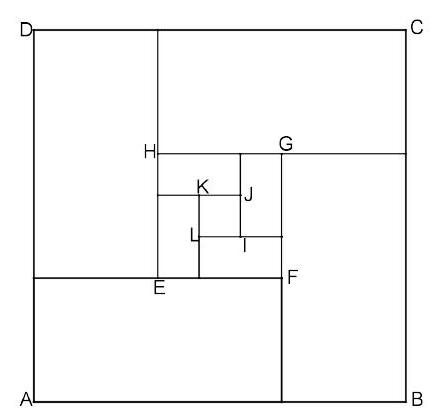
\includegraphics[max width=\textwidth, center]{2024_11_21_b57efd9a0a86eee00096g-1}

\section*{ZADANIE 2.}
W trójkącie równobocznym odcięto od jednego naroża trójkąt równoramienny, a od drugiego - trójkąt prostokątny tak, że pozostała część jest pięciokątem. Wyznacz miary kątów tego pięciokąta.

\section*{ZADANIE 3.}
Wojtek ma trzy patyczki: czerwony, zielony i niebieski. Ich długości to \(2 \mathrm{~cm}, 3 \mathrm{~cm}\) oraz 5 cm (kolejność tych liczb nie musi odpowiadać kolejności kolorów). Za pomocą każdego patyczka Wojtek zmierzył długość krawędzi stołu. Zielony patyk zmieścił się 75 razy, a niebieski 50 razy. Czerwony także zmieścił się całkowitą liczbę razy - ile?

\section*{ZADANIE 4.}
Wyznacz trzy kolejne liczby naturalne, których iloczyn jest sto razy większy od największej liczby czterocyfrowej.

\section*{ZADANIE 5.}
W Tłusty Czwartek mama kupiła mini-pączki dla swojej licznej rodzinki. Wojtek z Darkiem otrzymali trzecią część wszystkich i jeszcze trzy mini-pączki. Agnieszka z Basią wzięły trzecią część pozostałych i jeszcze dwa. Połowę pozostałych mini-pączków mama dała Jarkowi, a ostatnie sześć zjadła z tatą do kawy. Ile mini-pączków kupiła mama?


\end{document}